
%version 2: \usepackage{hyperref}


%%%%%%%%%%%%%%%%%%%%%%%%%%%%%%%%%%%%%%%%%%%%%%%%%%%%%%%%%%%%%%%%%%%%%%%%
%Para las ecuaciones siempre es Ec.(n).
%Para las figuras siempre es Fig.n, incluso en el caption de la figura. Tambien las Tablas
%Para las referencias es [n]
%%%%%%%%%%%%%%%%%%%%%%%%%%%%%%%%%%%%%%%%%%%%%%%%%%%%%%%%%%%%%%%%%%%%%%%%

\documentclass[
reprint,
%notitlepage,
%superscriptaddress,
%groupedaddress,
%unsortedaddress,
%runinaddress,
%frontmatterverbose, 
%preprint,
%showpacs,preprintnumbers,
%nofootinbib,
%nobibnotes,
%bibnotes,
%11 pt,
amsmath,
amssymb,
%aps,
%pra,
prb,
%rmp,
%tightenlines %esto hizo el milagro de sacar los espacios en blancos estocásticos (?)
%prstab,
%prstper,
%floatfix,\textbf{}
]{revtex4-1} %Instalar primero para usarlo. Paquete malo.

%\documentclass[onecolumn, aps, amsmath,amssymb ]{article}
\usepackage{lipsum}  
\usepackage{graphicx}% Include figure files
\usepackage{subfig}
\usepackage{braket}
\usepackage{comment} %comment large chunks of text
\usepackage{dcolumn}% Align table columns on decimal point
\usepackage{bm}% bold math
%\usepackage{hyperref}% add hypertext capabilities
\usepackage[mathlines]{lineno}% Enable numbering of text and display math
%\linenumbers\relax % Commence numbering lines
\usepackage{mathtools} %% Para el supraíndice

\usepackage[nice]{nicefrac}

%%%%%%%El Señor Español%%%%%%%%%%%%%%%%%%%%%%%%%%%
\usepackage[utf8]{inputenc} %acento
\usepackage[
spanish, %El lenguaje.
es-tabla, %La tabla y no cuadro.
activeacute, %El acento.
es-nodecimaldot %Punto y no coma con separador de números
]{babel}
\usepackage{microtype} %para hacerlo más bonito :33 como vos (?) 
%%%%%%%%%%%%%%%%%%%%%%%%%%%%%%%%%%%%%%%%%%%%%%%%%%%
%%%%%%%%% Para que las imágenes se queden dónde las quiero (?
\usepackage{float}
%%%%%%%%%%
\usepackage{enumitem}
\usepackage{hyperref} % Para usar \url

%%%%%%%%Cambia a Fig de Figure%%%%%%%%%%
\makeatletter
\renewcommand{\fnum@figure}{Fig. \thefigure} 
\makeatother
%%%%%%%%%%%%%%%%%%%%%%%%%%%%%%%%%%%%%%%%
\raggedbottom



   %\usepackage[caption=false]{subcaption}

\begin{document}
%%%%%%%%%%%%%%%%%%%%%%%%%%%%%%%%%%Título%%%%%%%%%%%%%%%%%%%%%%%%%%%%%%%%%%%%%%
%%%%%%%%%%%%%%%%%%%%%%%%%%%%%%%%%%%%%%%%%%%%%%%%%%%%%%%%%%%%%%%%%%%%%%%%%%%%%%

\title{Práctica 1: Redes Neuronales y Aprendizaje Profundo para Visión Artificial}
\author{Evelyn~G.~Coronel}

\affiliation{
Aprendizaje Profundo y Redes Neuronales Artificiales\\ Instituto Balseiro\\}

\date[]{\lowercase{\today}} %%lw para lw, [] sin date


\maketitle
%\onecolumngrid


\section*{Ejercicio 1}

En este ejercicio se implementó una regresión lineal de la función $f(x_i)= \sum_{i=1}^d a_{i}x_i+ b $ para un cantidad N de puntos en d dimensiones.  Para realizar este ejercicio se generan datos de forma aleatoria para los valores de $x_i$ y $a_{m,exacto}$, se calcula el valor $y_i=f(x_i) + \epsilon$ con un ruido uniforme, y utiliza la ecuación

\begin{equation}
     \vec a = (X^TX)^{-1}X^T \vec y,
     \label{eq:ejer1}
 \end{equation} 
con $\vec a$ representa a $\{a_i, b\}$  y $X$ son los valores de $x_i$ escrita en forma matricial.


%En las figuras \ref{fig:ejer1_a_ejemplos}, \ref{fig:ejer1_a_porcentaje}, \ref{fig:ejer1_y_ejemplos} y \ref{fig:ejer1_y_porcentaje} se muestran los errores cuadráticos medios en función de la dimensión de los parámetros obtenidos en la regresión con respecto a los parámetros exactos, así como también el error asociado a salida de la función $f(x)$ de datos de prueba. 

%En las Figs. \ref{fig:ejer1_a_porcentaje} y \ref{fig:ejer1_y_porcentaje} se muestran los errores cuadráticos medios en función de la dimensión de los parámetros obtenidos en la regresión con respecto a los parámetros exactos, así como también el error asociado a salida de la función $f(x)$ de datos de prueba. En estas figuras se muestran distintas cantidades de ejemplos para calcular los coeficientes, por ejemplo la línea indicada como 1.5 muestra el error cuadrático medio (MSE) en función de la dimensión $d$ del problema, cuando se calculan los coeficientes con $N=1.5d$ ejemplos.  Si nos fijamos en dos dimensiones  en particular, por ejemplo en $d_1=40$ y en $d_2=120$. Cuando nos movemos sobre el eje $y$, el MSE aumenta cuando menos ejemplos tomamos para entrenar. 

En las Figs.  \ref{fig:ejer1_a_ejemplos} y \ref{fig:ejer1_y_ejemplos}  e muestran los errores cuadráticos medios  (MSE) en función de la cantidad de ejemplos dados para calcular los parámetros del problema. Aunque 

si comparamos los errores  


%En las Figs. \ref{fig:ejer1_a_ejemplos} y \ref{fig:ejer1_y_ejemplos} se mantienen el valor de N. Cada línea indica la cantidad de ejemplos usados para calcular los parámetros $\{a_i, b\}$ . A medida que se aumenta la cantidad de ejemplos, el error en los parámetros y la salida aumenta, esto se debe a la Ec. \ref{eq:ejer1} que se basa





    \begin{figure}[H]
        \centering
        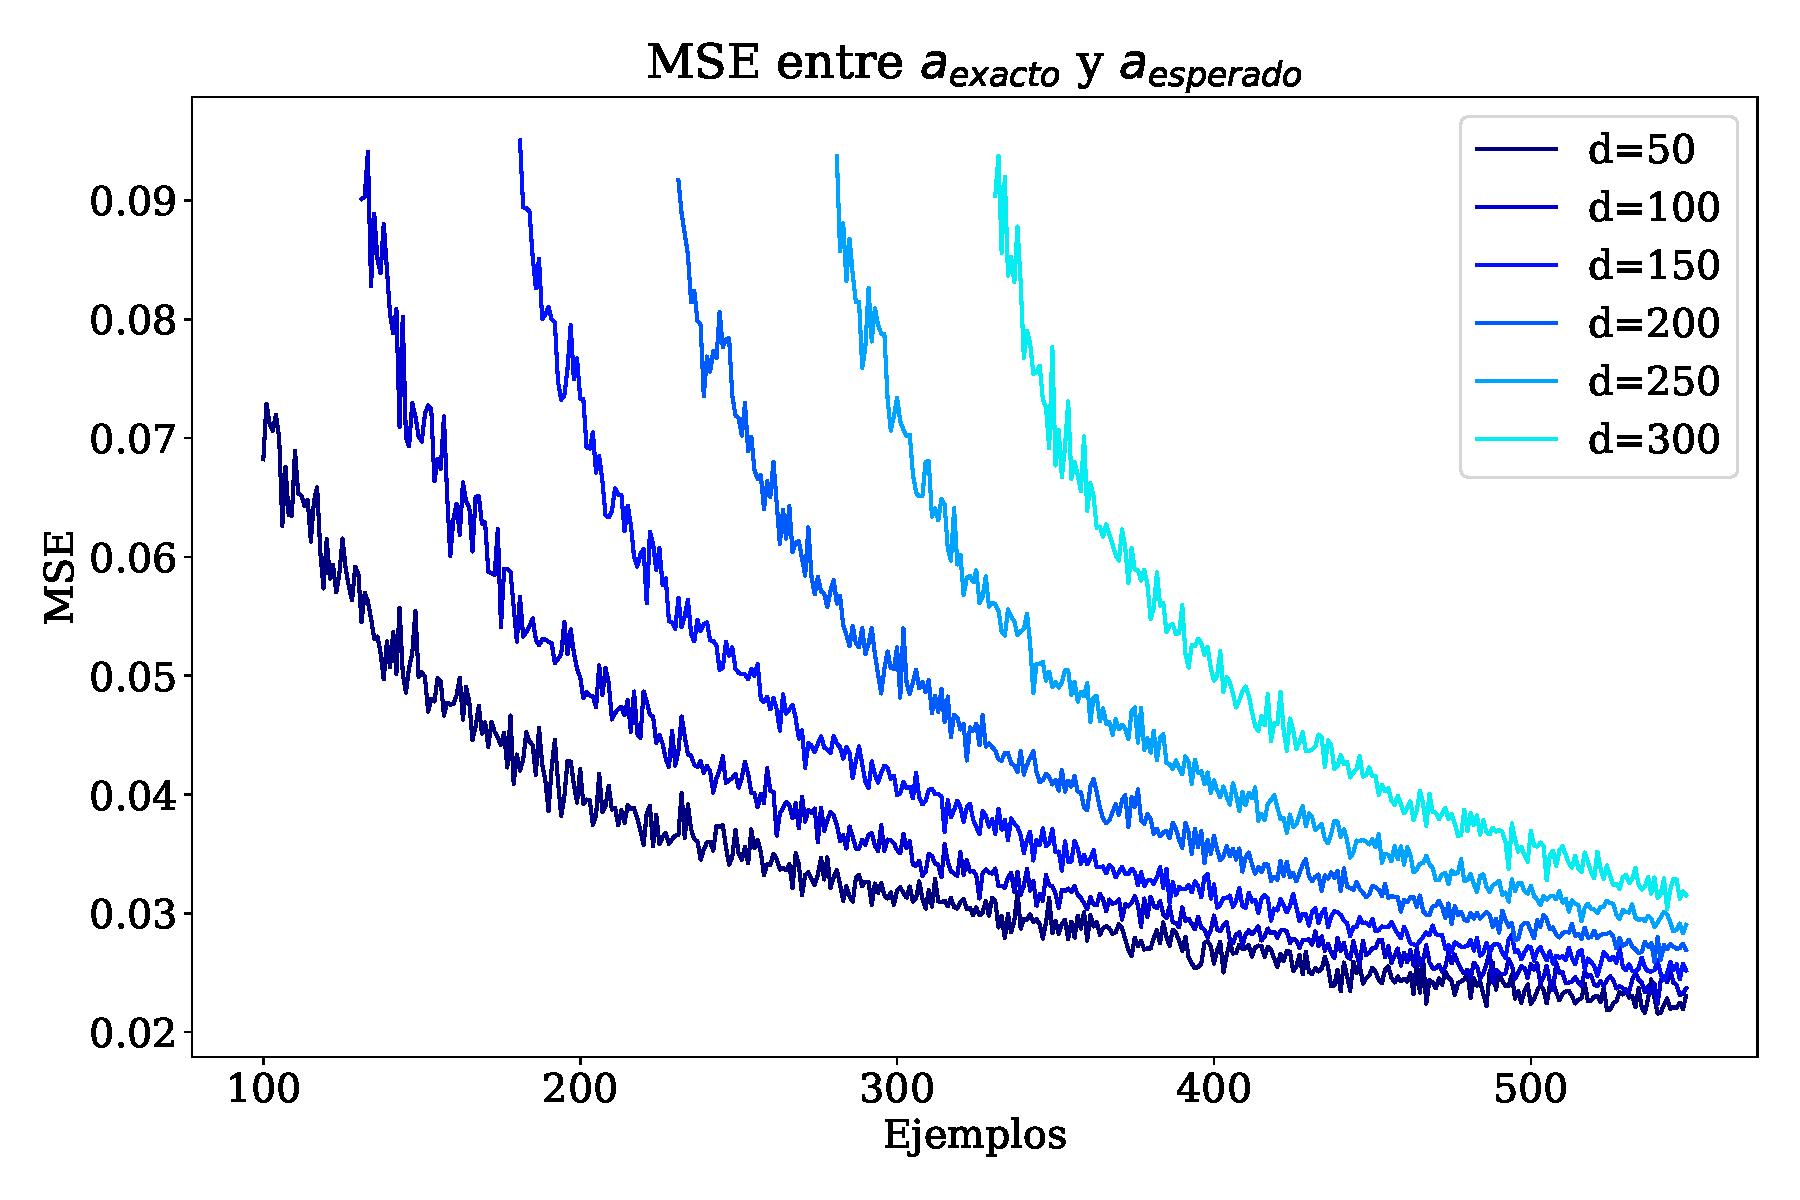
\includegraphics[width=0.49\textwidth]{plots/ejer_1_mse_a_ejemplos.pdf}
        \caption{ejemplos}
        \label{fig:ejer1_a_ejemplos}
    \end{figure}

    % \begin{figure}[H]
    %     \centering
    %     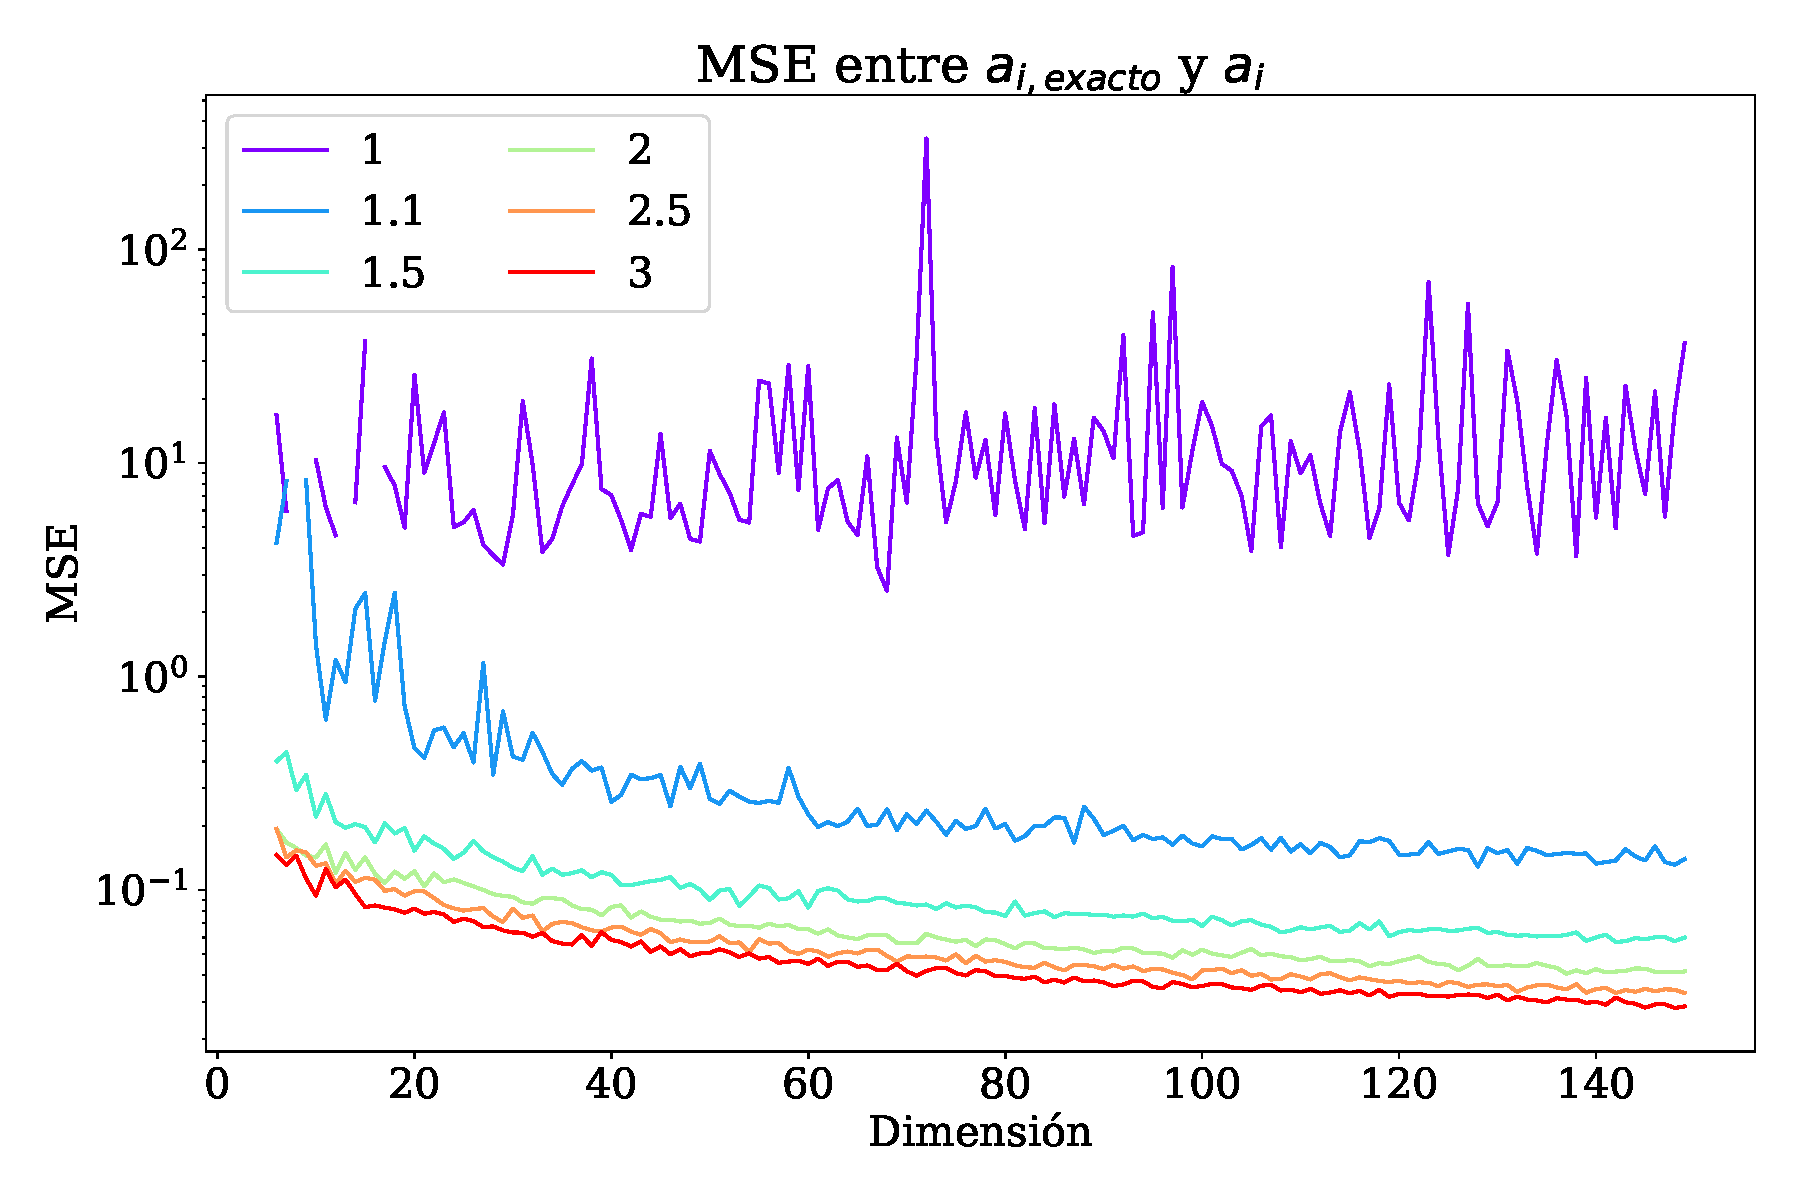
\includegraphics[width=0.5\textwidth]{plots/ejer_1_mse_a_porcentaje.pdf}
    %     \caption{ejemplos}
    %     \label{fig:ejer1_a_porcentaje}
    % \end{figure}

    \begin{figure}[H]
        \centering
        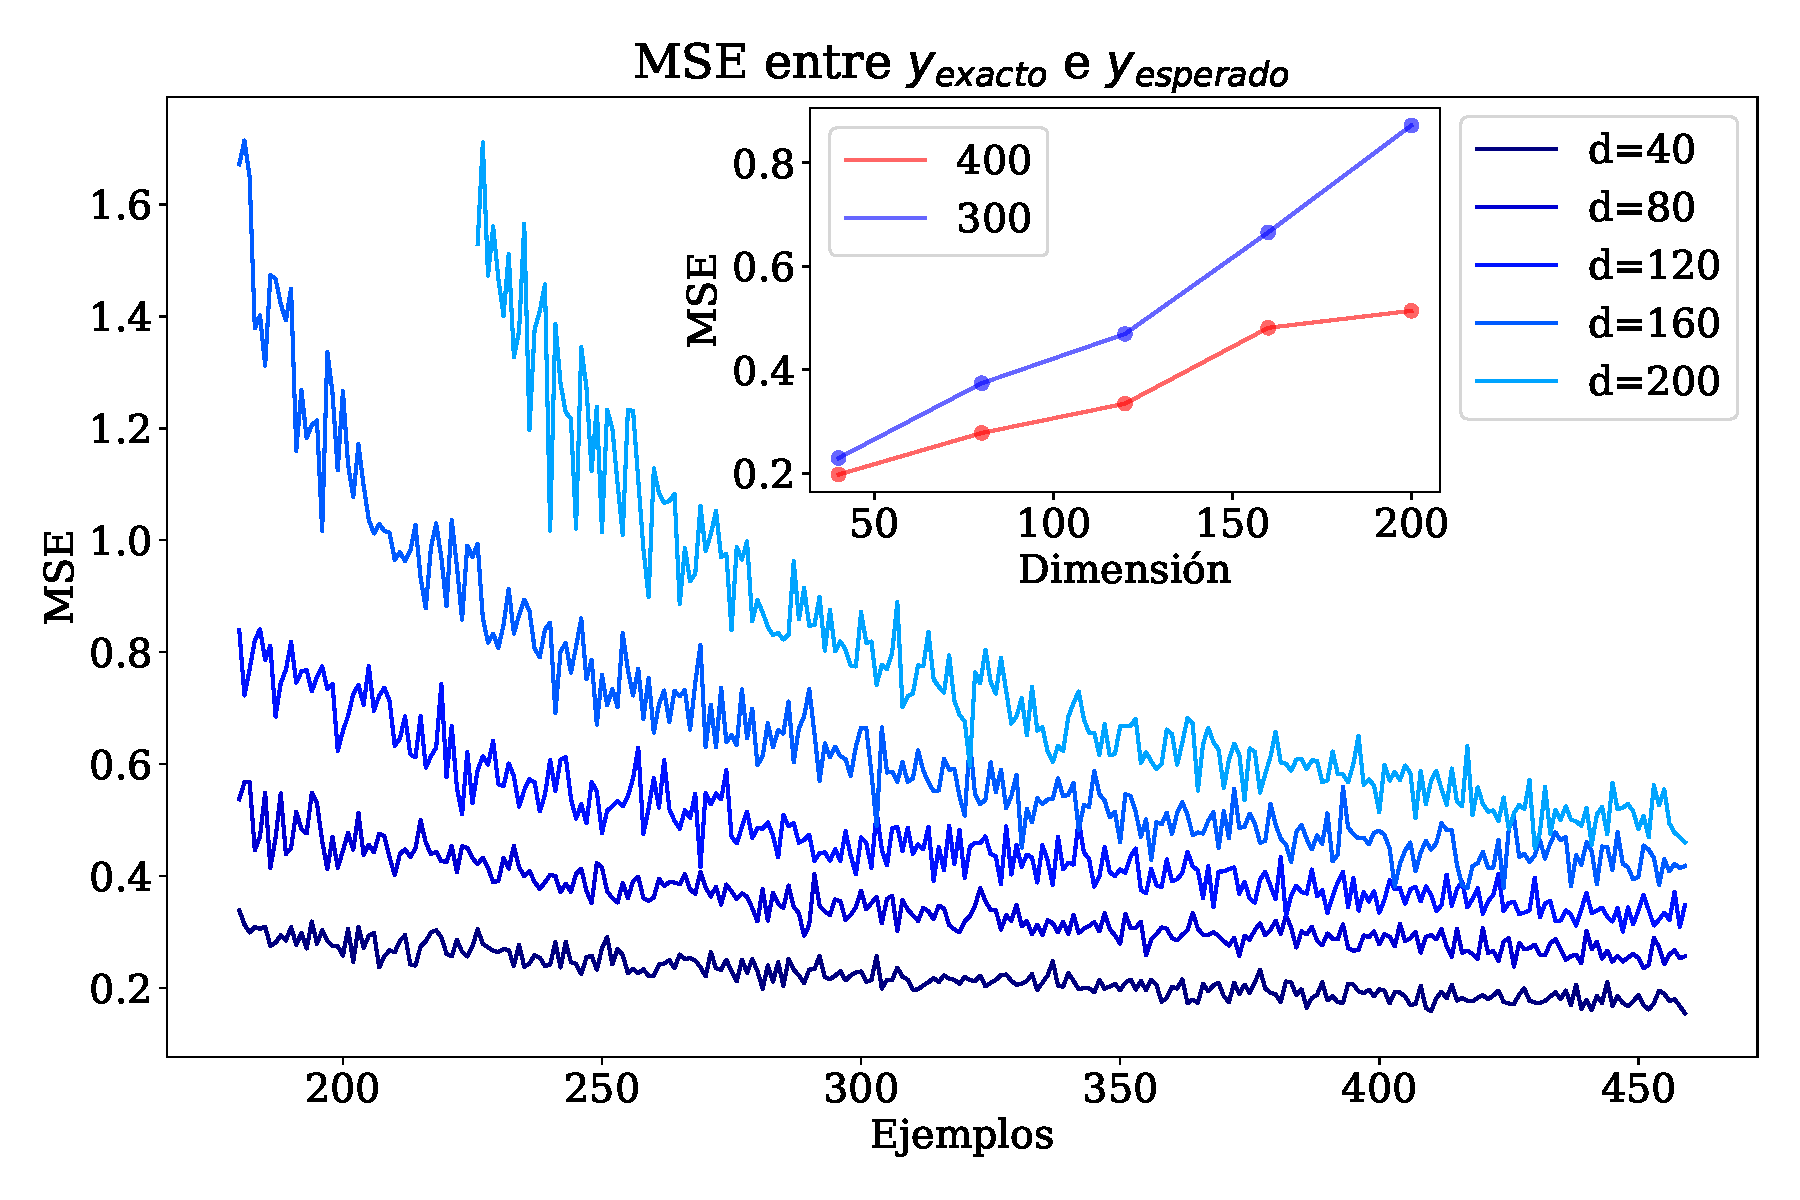
\includegraphics[width=0.5\textwidth]{plots/ejer_1_mse_y_ejemplos.pdf}
        \caption{ejemplos}
        \label{fig:ejer1_y_ejemplos}
    \end{figure}

    % \begin{figure}[H]
    %     \centering
    %     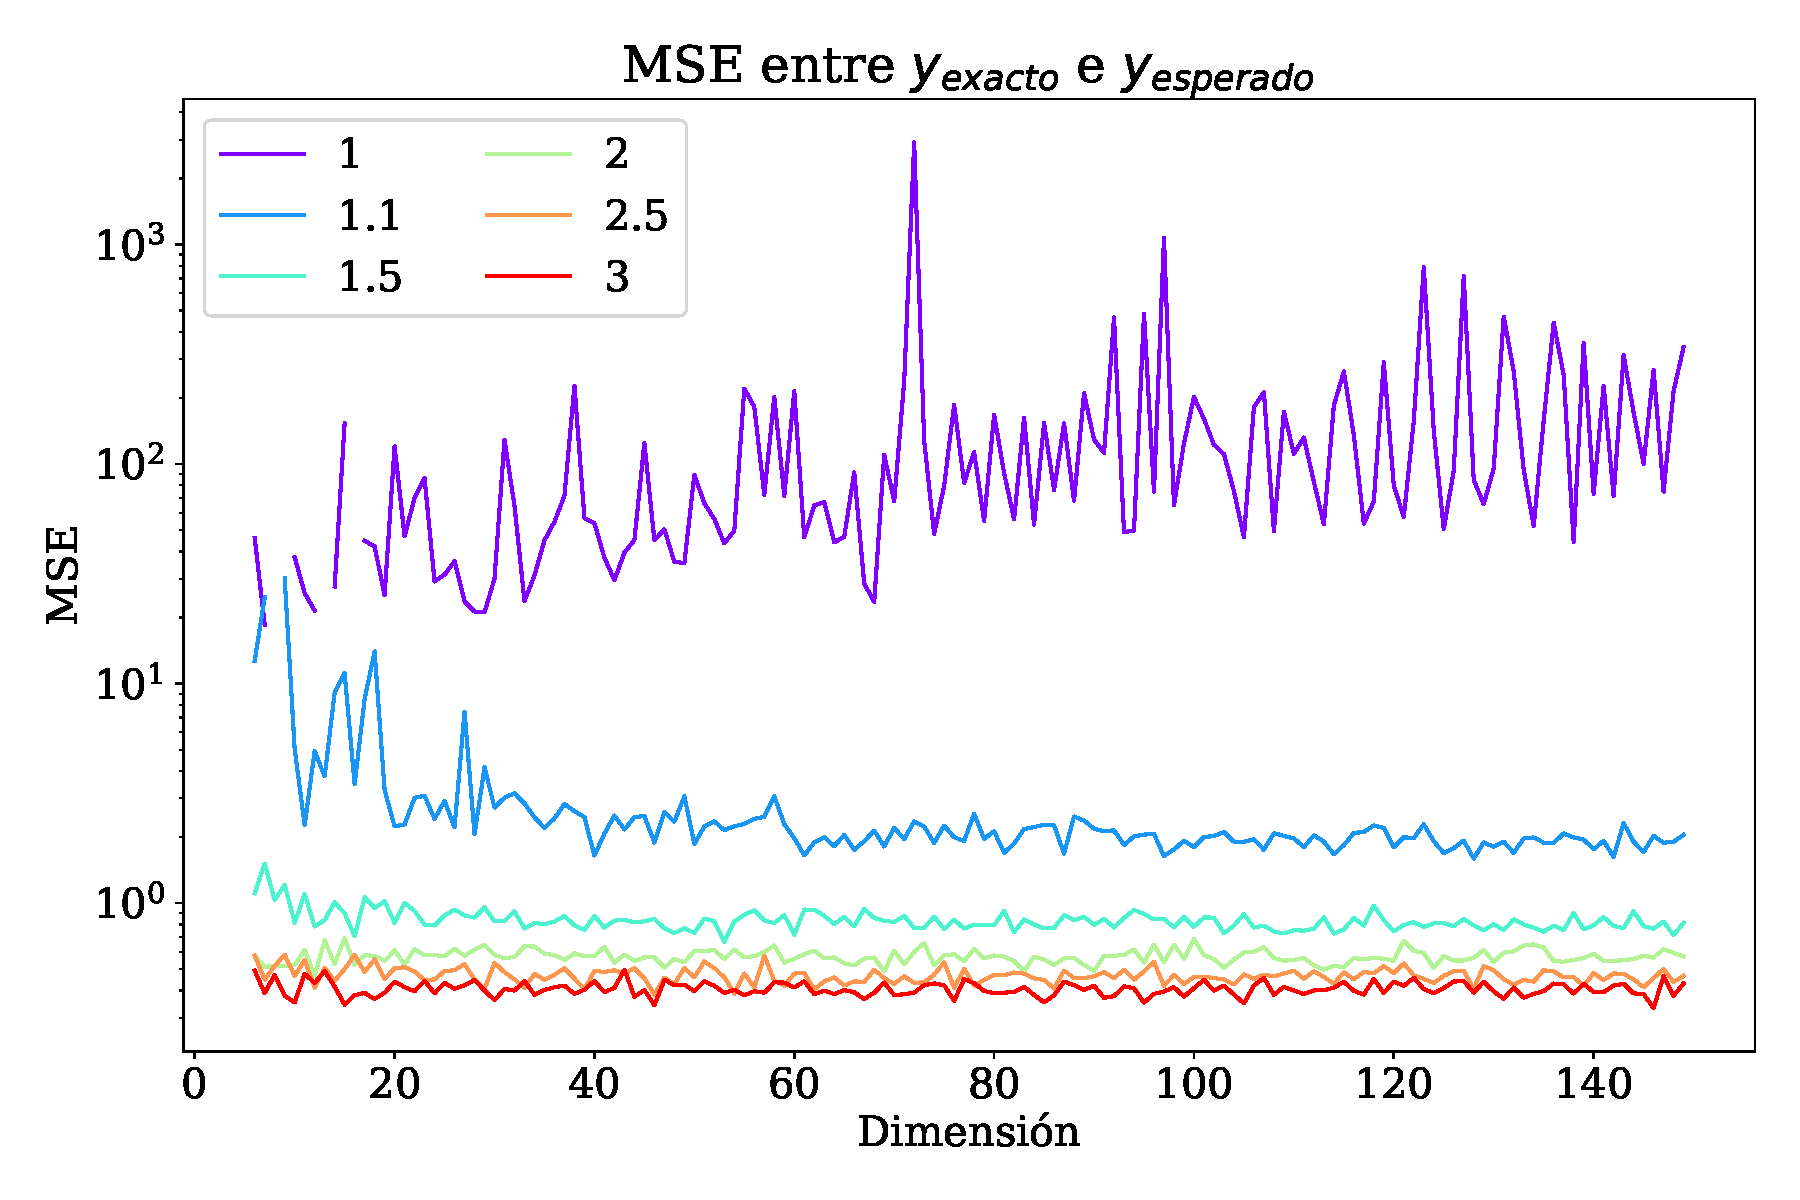
\includegraphics[width=0.5\textwidth]{plots/ejer_1_mse_y_porcentaje.pdf}
    %     \caption{ejemplos}
    %     \label{fig:ejer1_y_porcentaje}
    % \end{figure}


    \section*{Ejercicio 2}

    Las medias y las desviaciones estandar de cada clase fueron inicializadas de manera aleatoria

    Los gráficos se hicieron con d=7 y p=4


    Esto es un ejemplo que converge
    \begin{figure}[H]
        \centering
        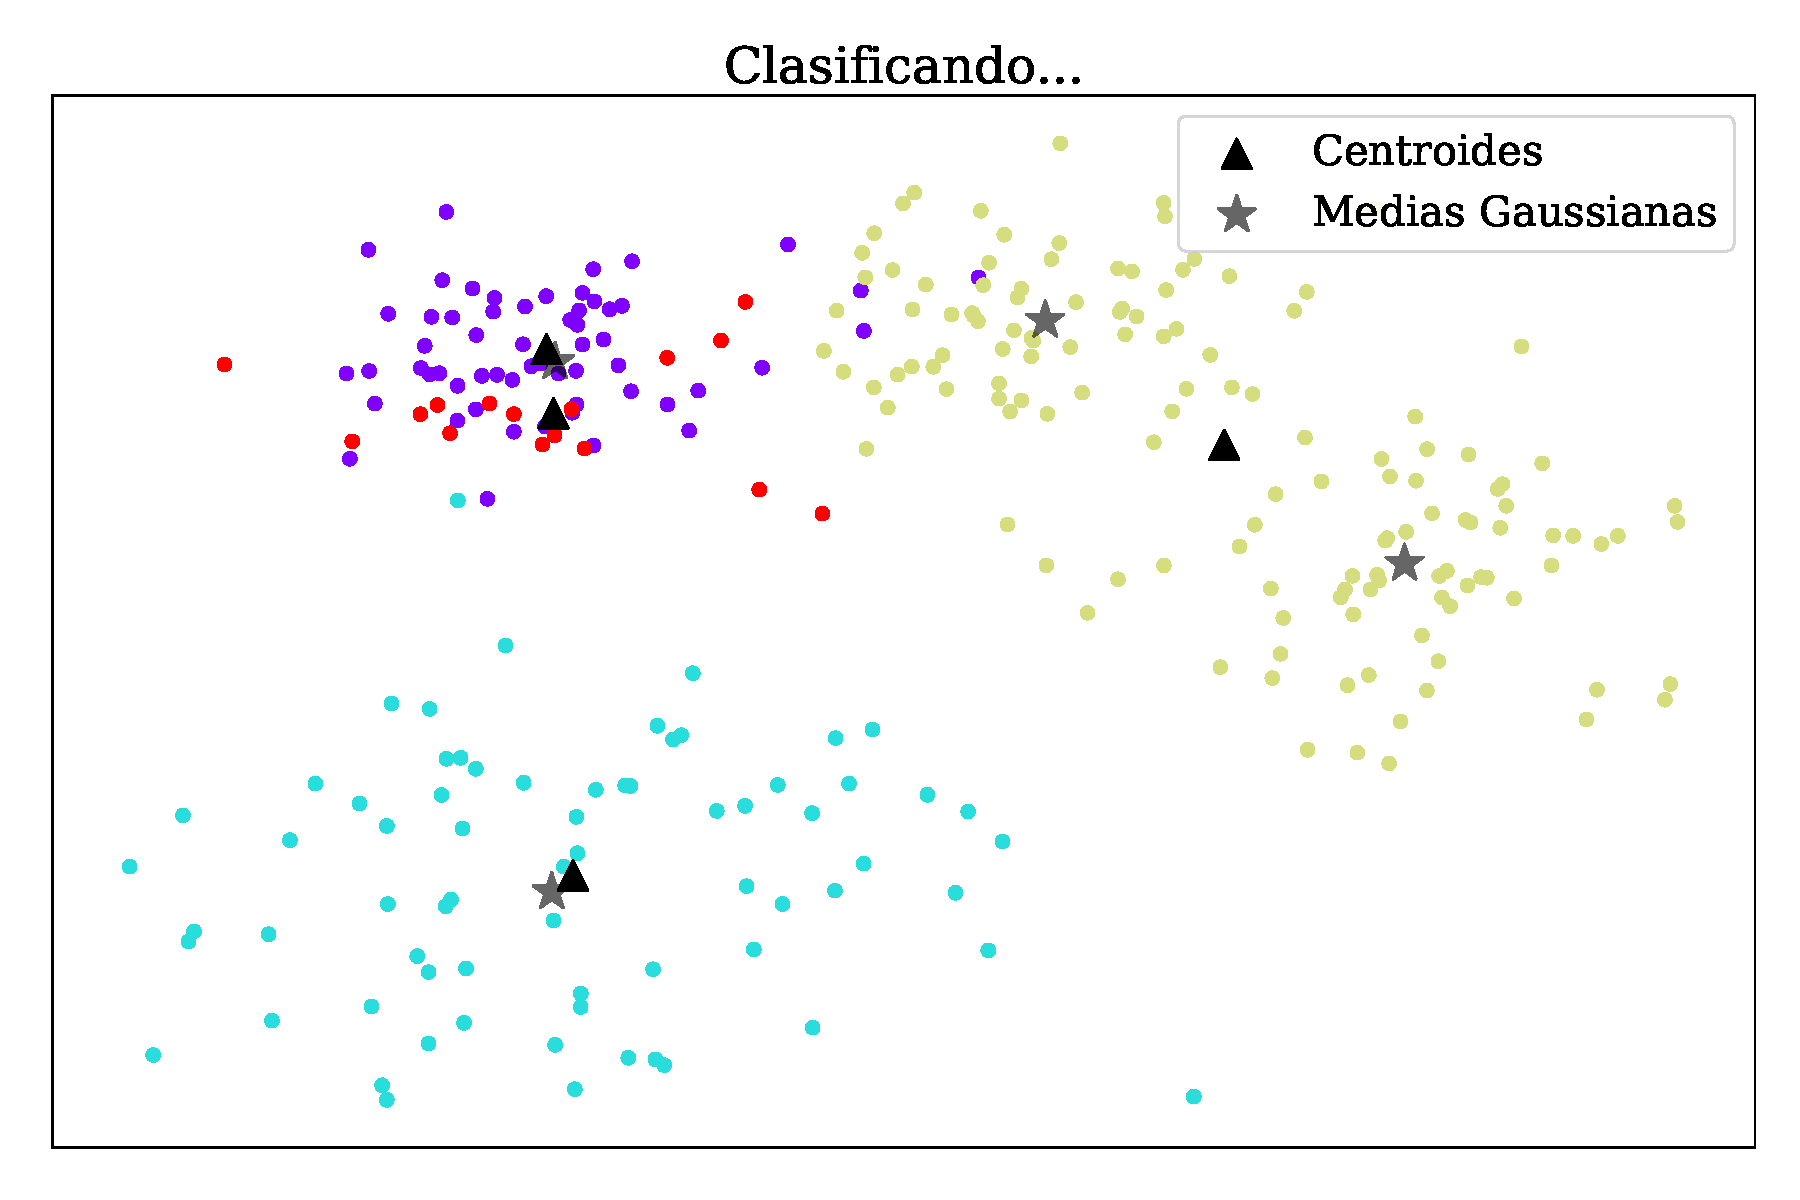
\includegraphics[width=0.5\textwidth]{plots/ejer_2_clasificando_a_conv.pdf}
        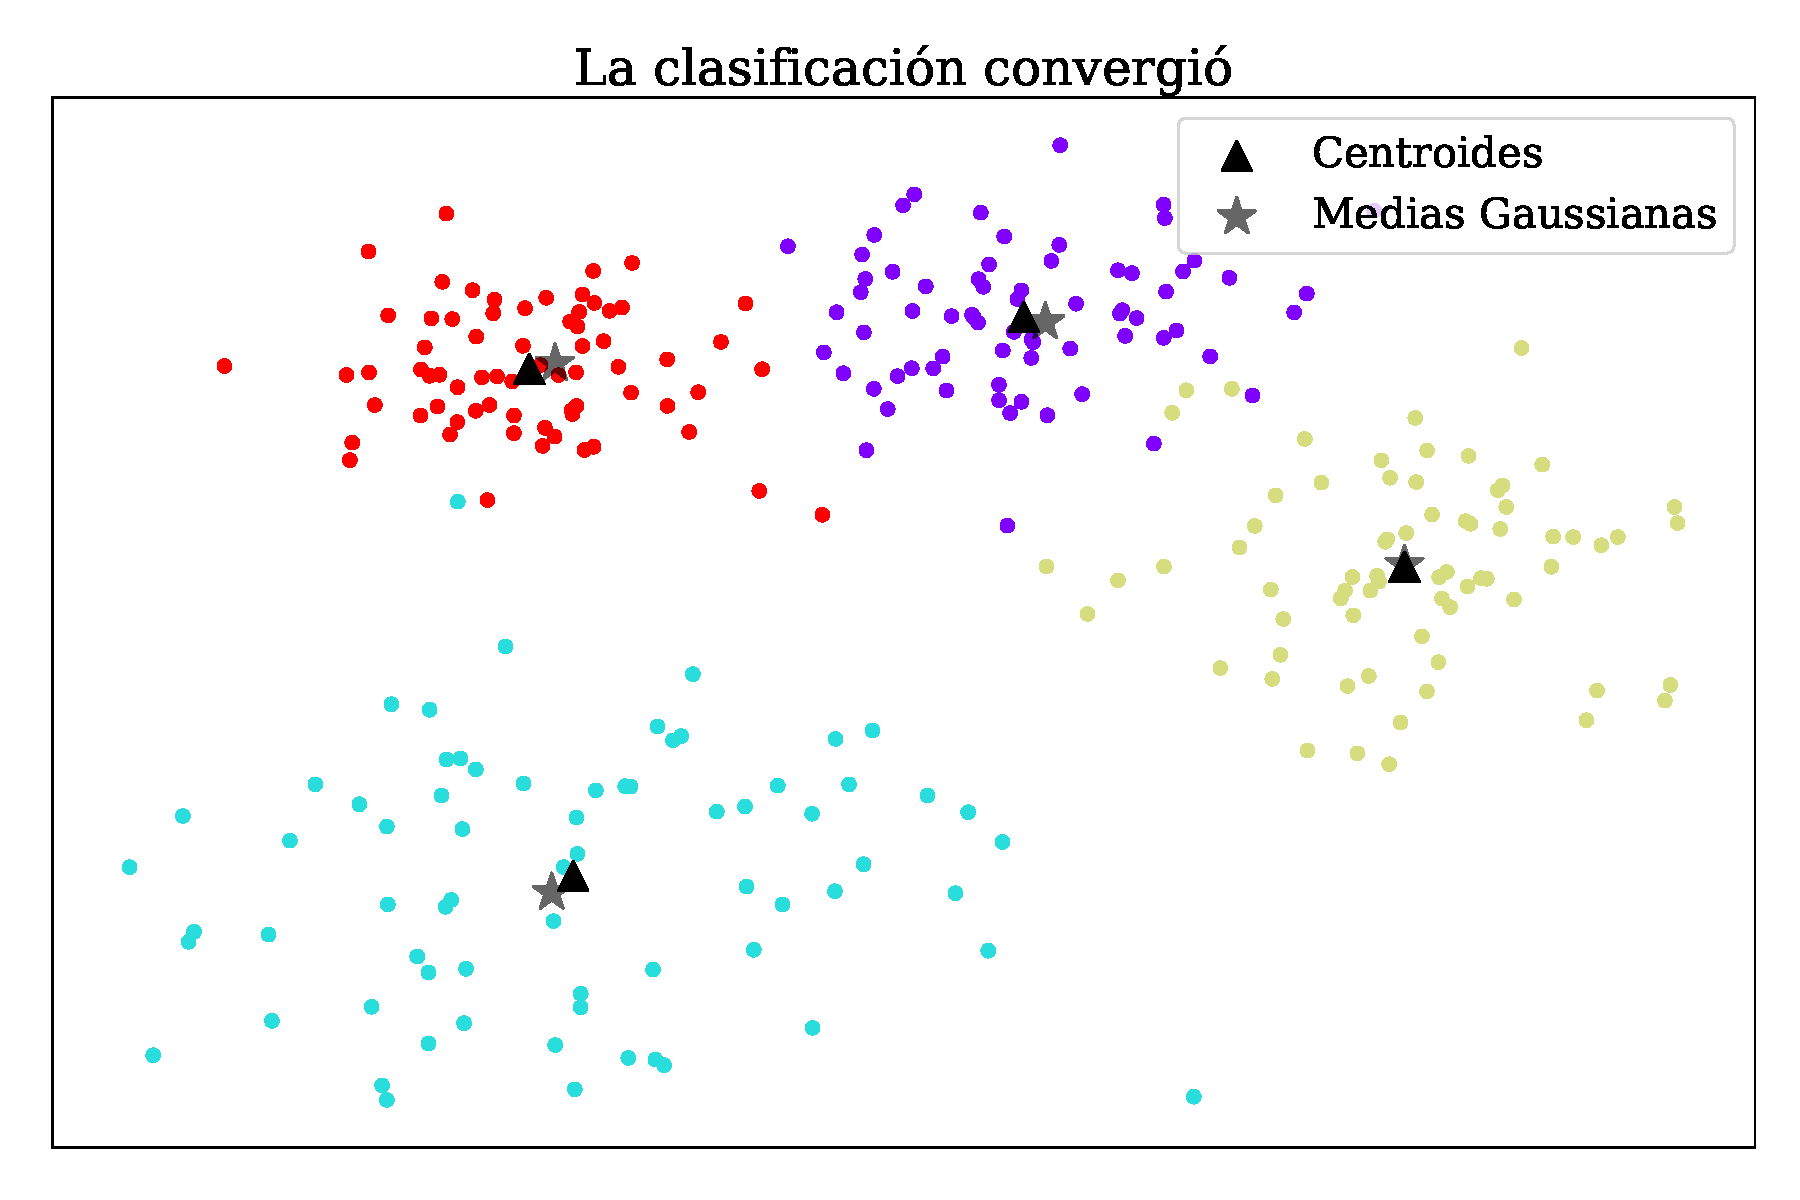
\includegraphics[width=0.5\textwidth]{plots/ejer_2_si_converge.pdf}
        \caption{ejemplos}
        \label{fig:ejer2_converge}
    \end{figure}

    Este es un ejemplo donde no funciona

    \begin{figure}[H]
        \centering
        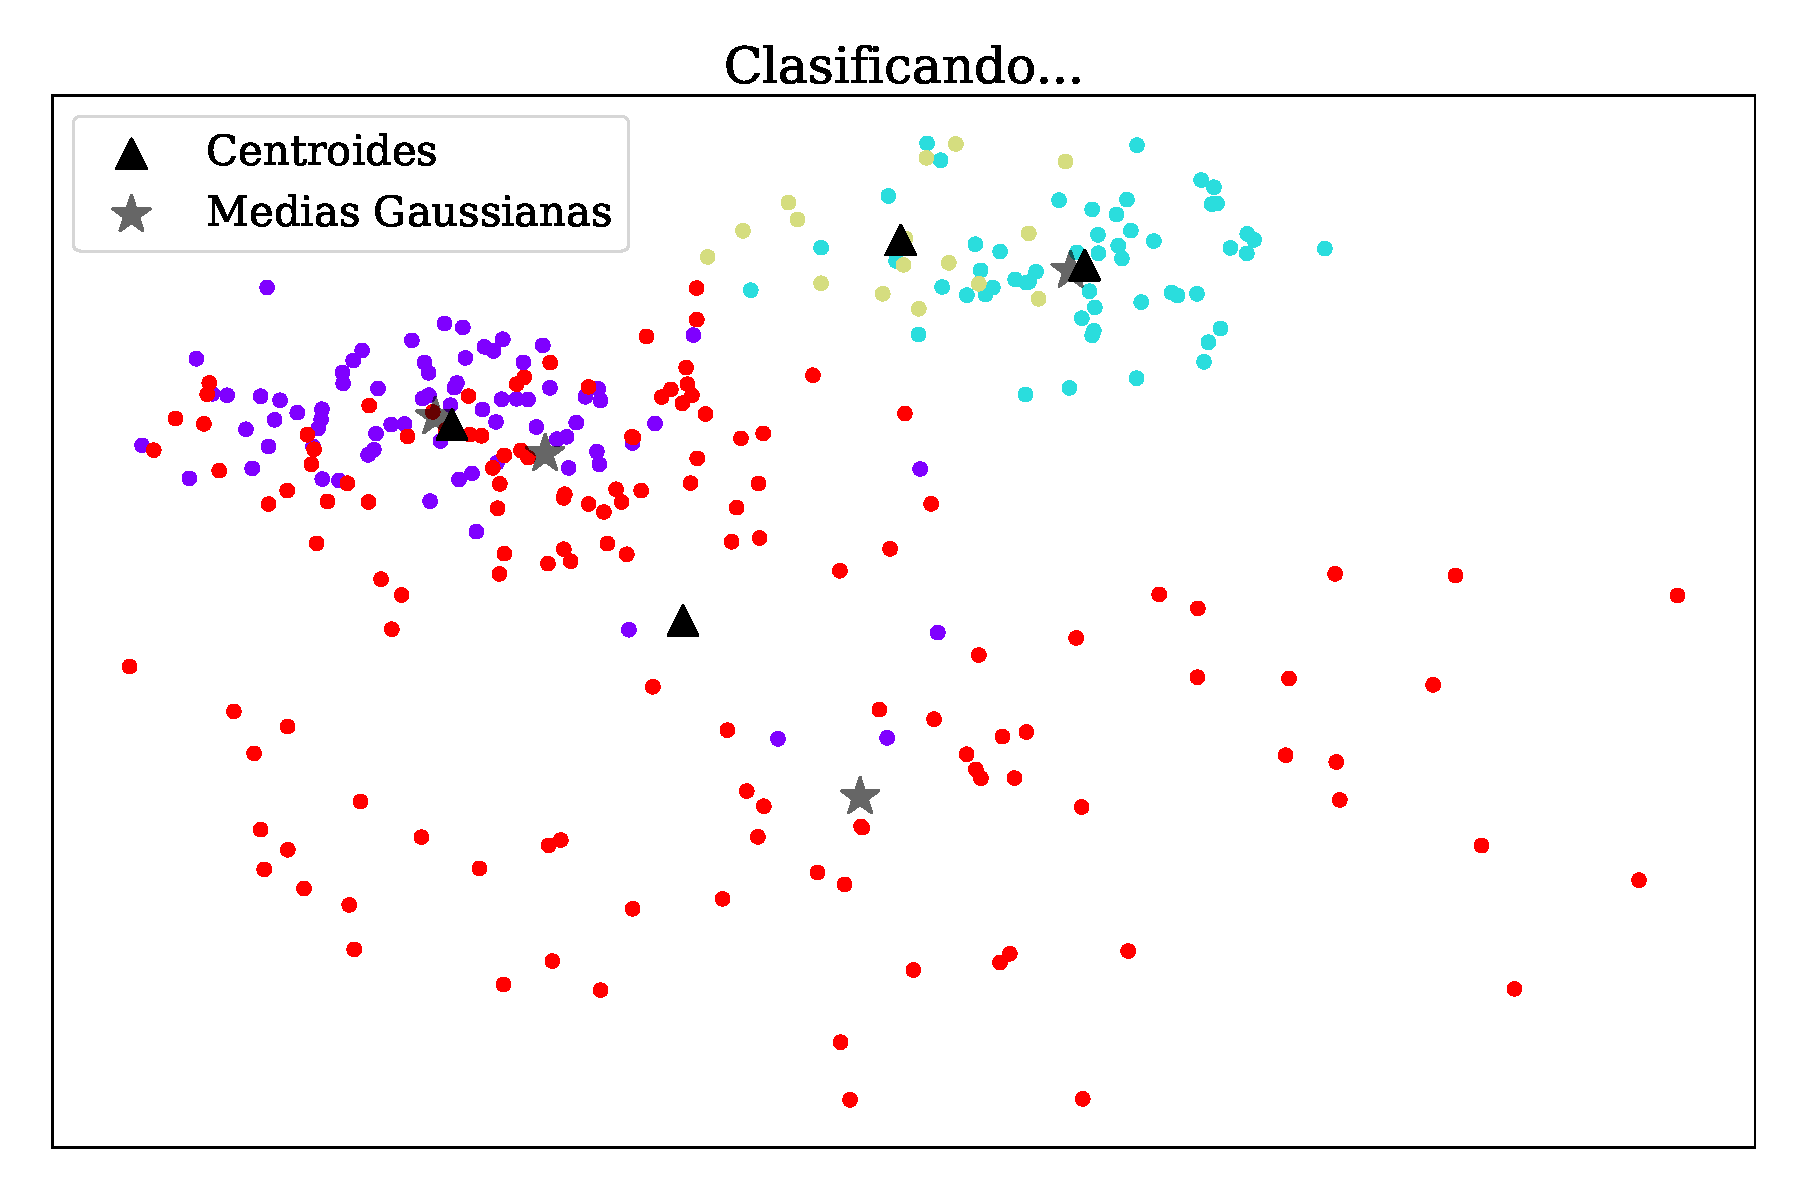
\includegraphics[width=0.5\textwidth]{plots/ejer_2_clasificando.pdf}
        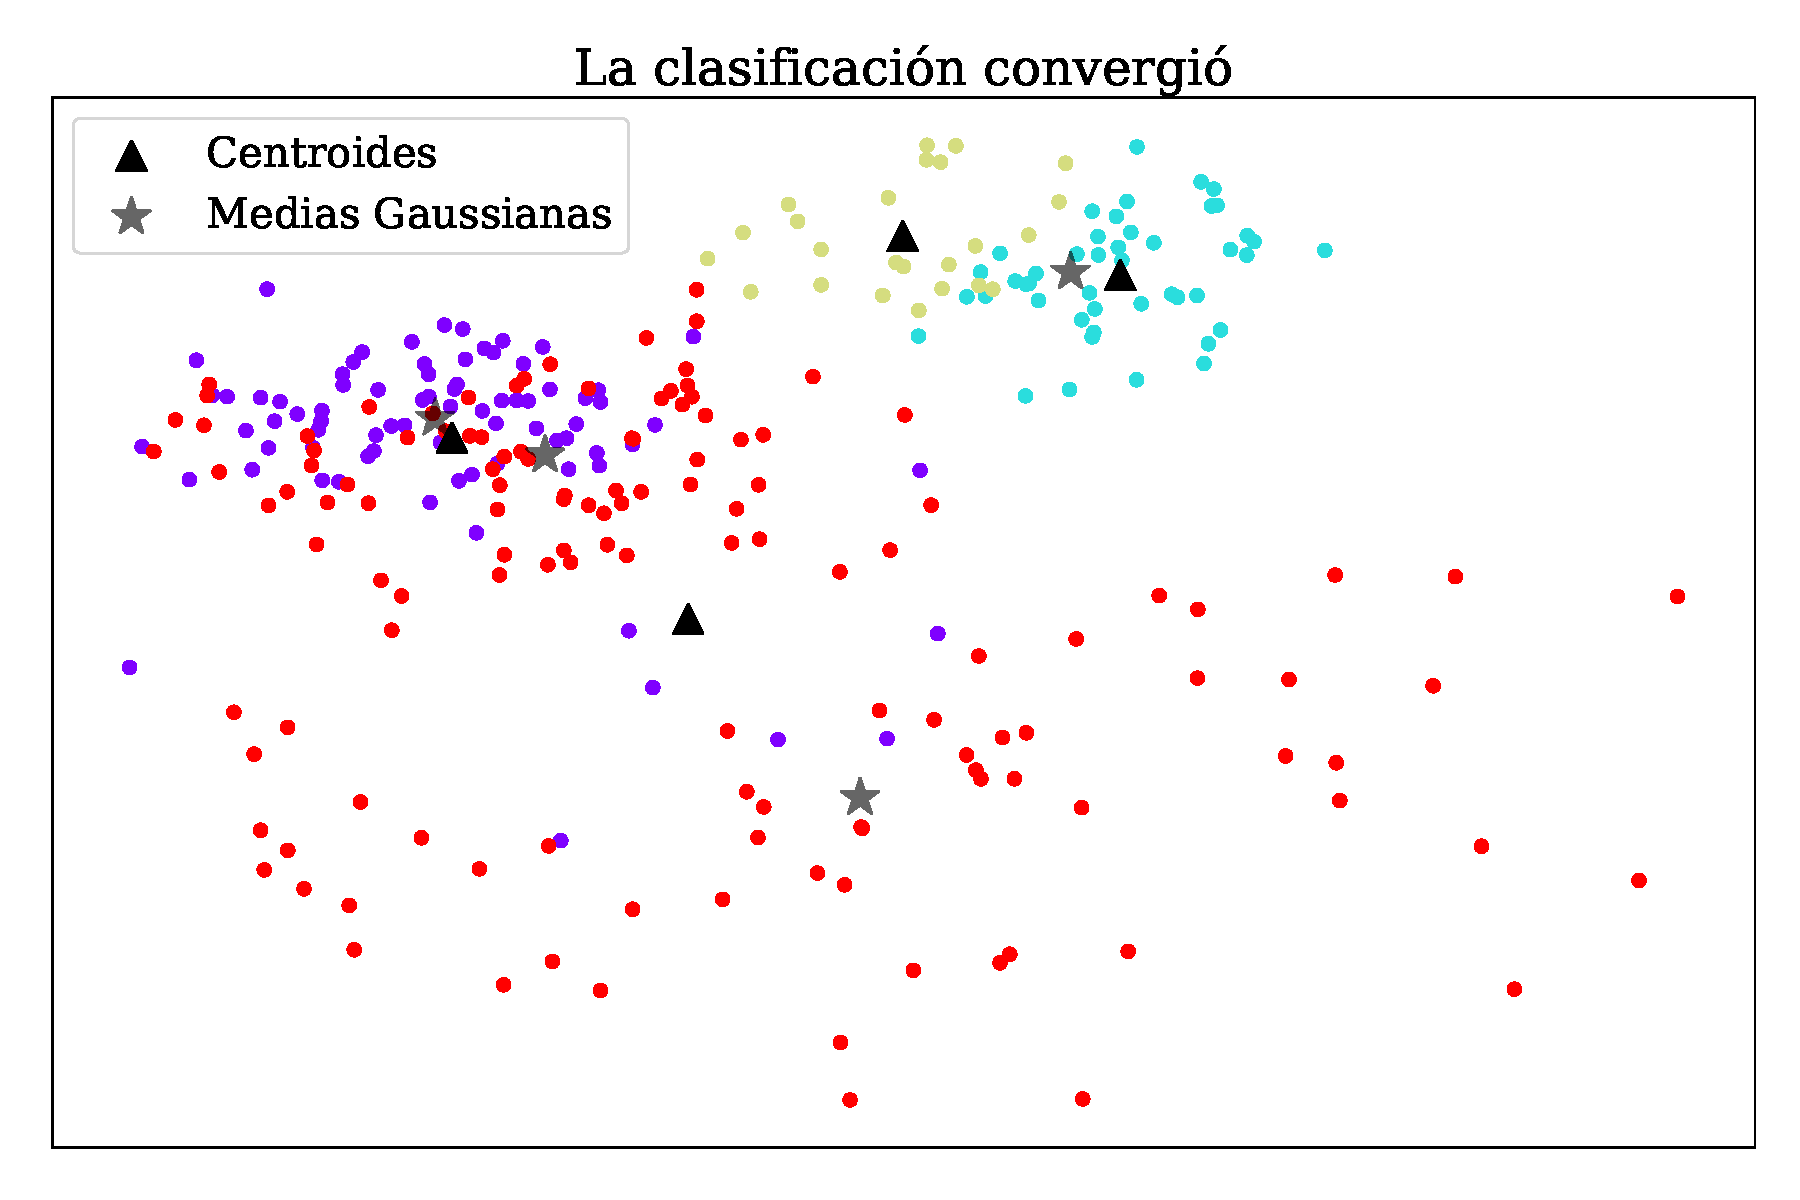
\includegraphics[width=0.5\textwidth]{plots/ejer_2_no_converge.pdf}
        \caption{ejemplos}
        \label{fig:ejer2_no_converge}
    \end{figure}

   \section*{Ejercicio 3}


    \section*{Ejercicio 4}


k=1
Dimensiones del set de entrenamiento  (375, 2)
375 ejemplos de entrenamiento
125 ejemplos para probar

36.0\% probando con 125 ejemplos

\begin{figure}[H]
    \centering
    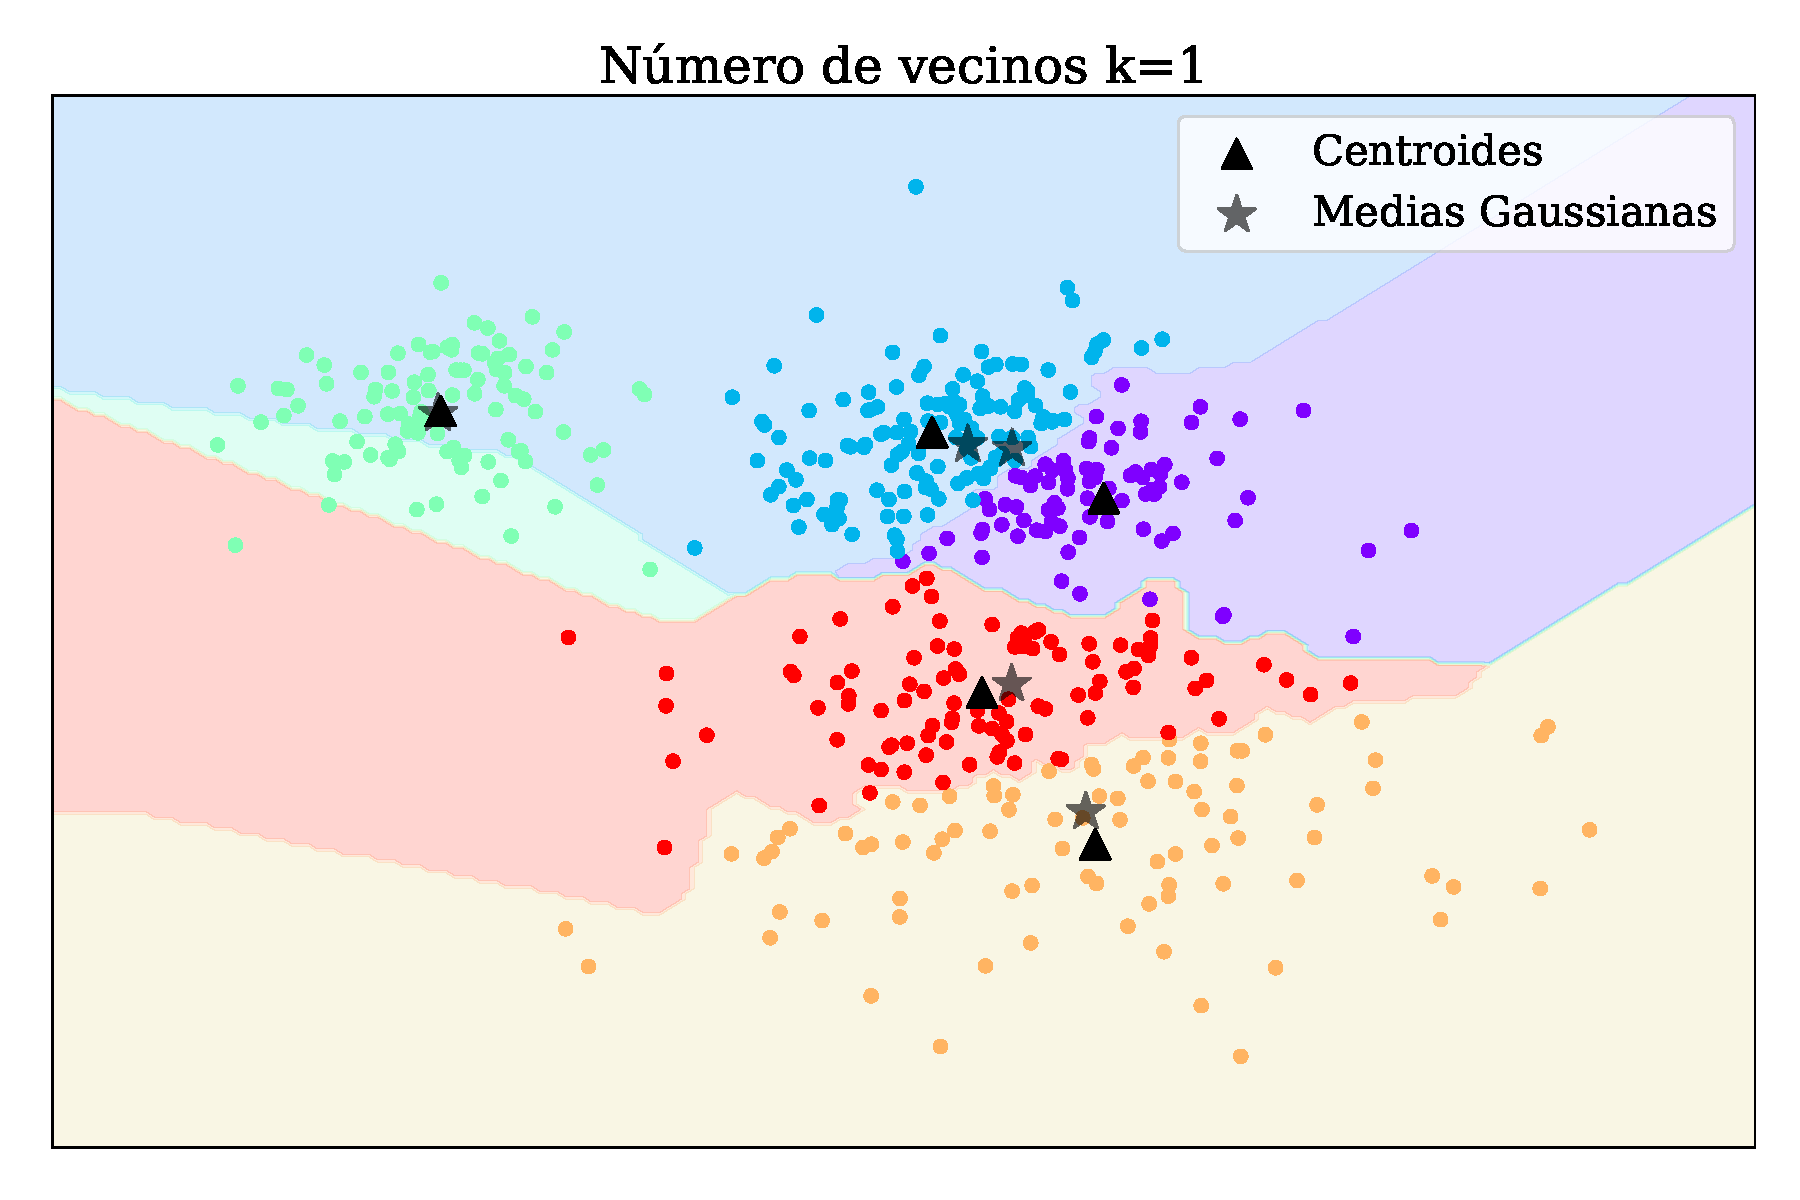
\includegraphics[width=0.5\textwidth]{plots/ejer_4_K-1_no_coverge.pdf}
    \caption{K=1 malo}
    \label{fig:ejer4_k_1_malo}
\end{figure} 

k=1
Dimensiones del set de entrenamiento  (375, 2)
375 ejemplos de entrenamiento
125 ejemplos para probar

99.2\% probando con 125 ejemplos

\begin{figure}[H]
    \centering
    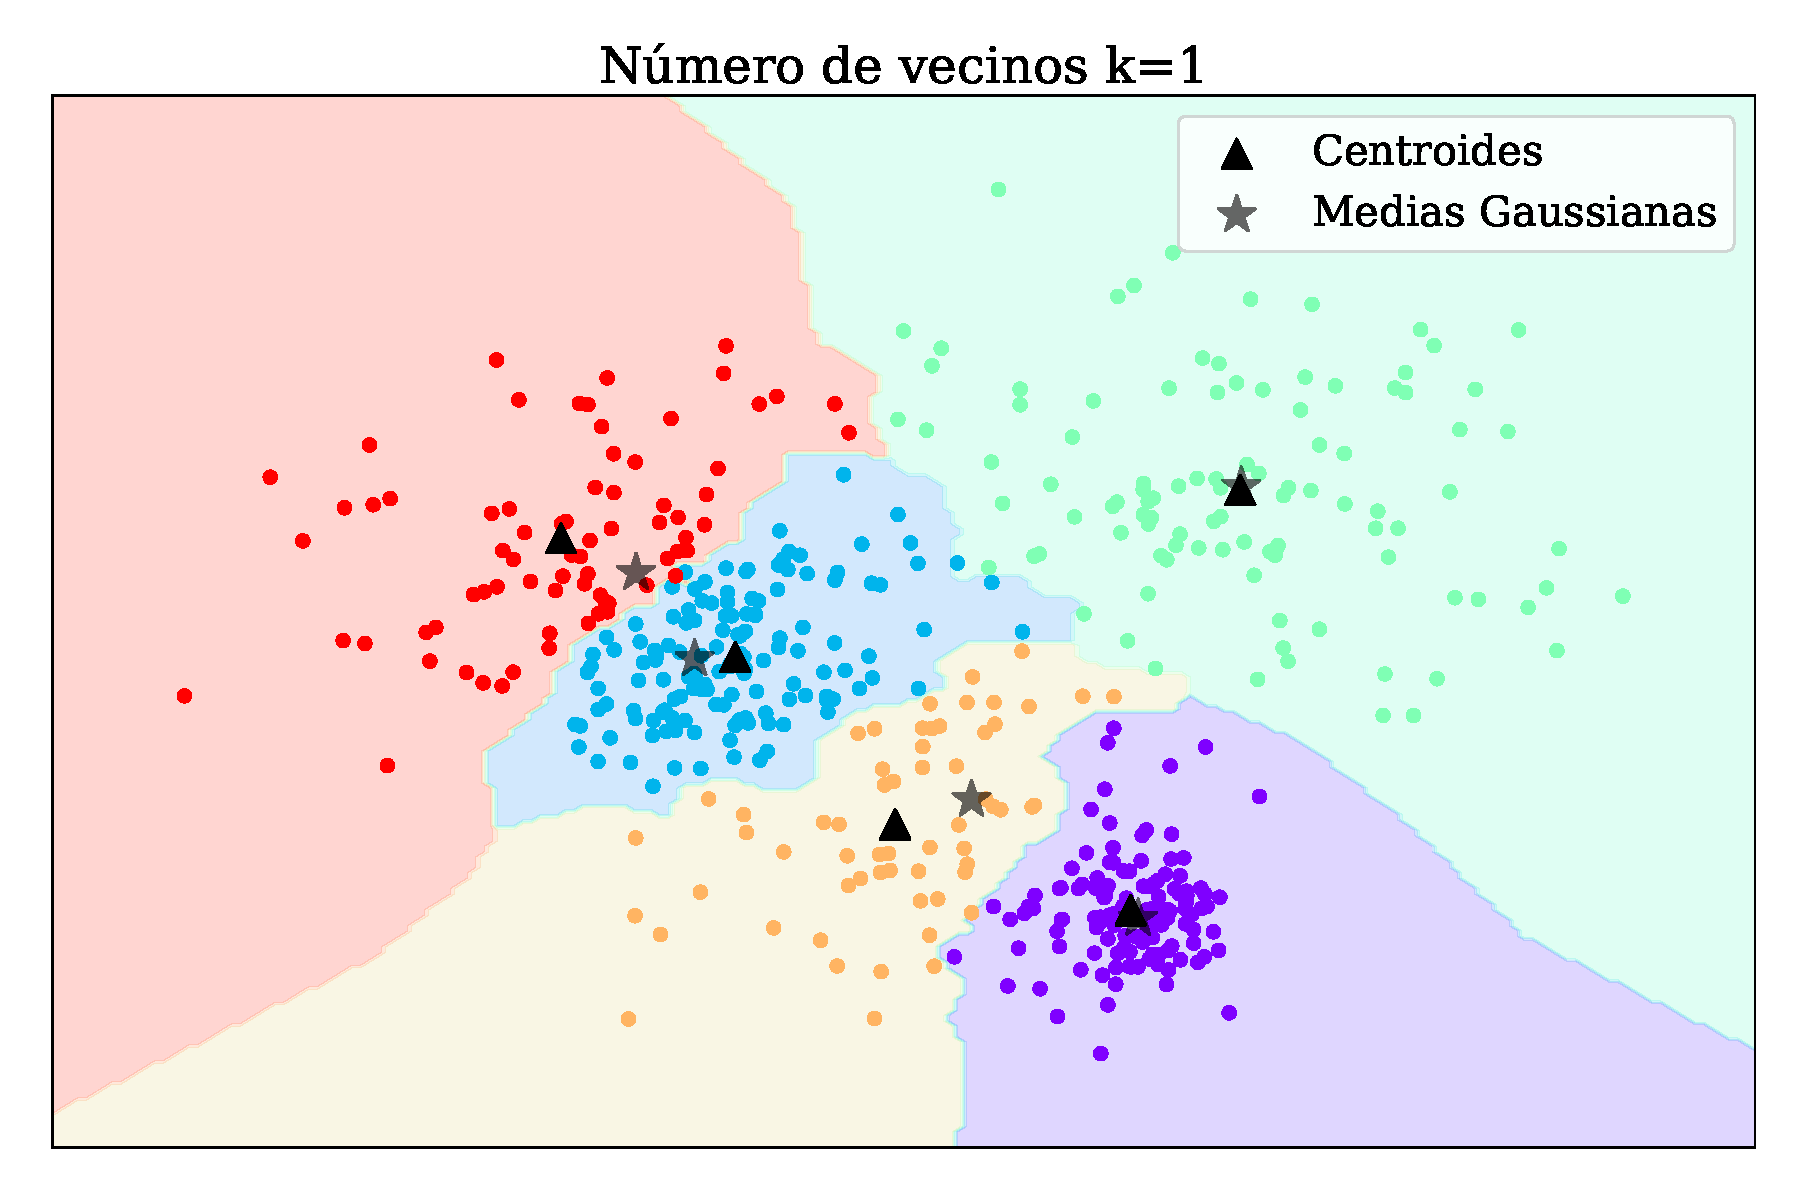
\includegraphics[width=0.5\textwidth]{plots/ejer_4_K-1_si_converge.pdf}
    \caption{K=1 malo}
    \label{fig:ejer4_k_1}
\end{figure} 


k=3
Dimensiones del set de entrenamiento  (375, 2)
375 ejemplos de entrenamiento
125 ejemplos para probar

94.4\% probando con 125 ejemplos

\begin{figure}[H]
    \centering
    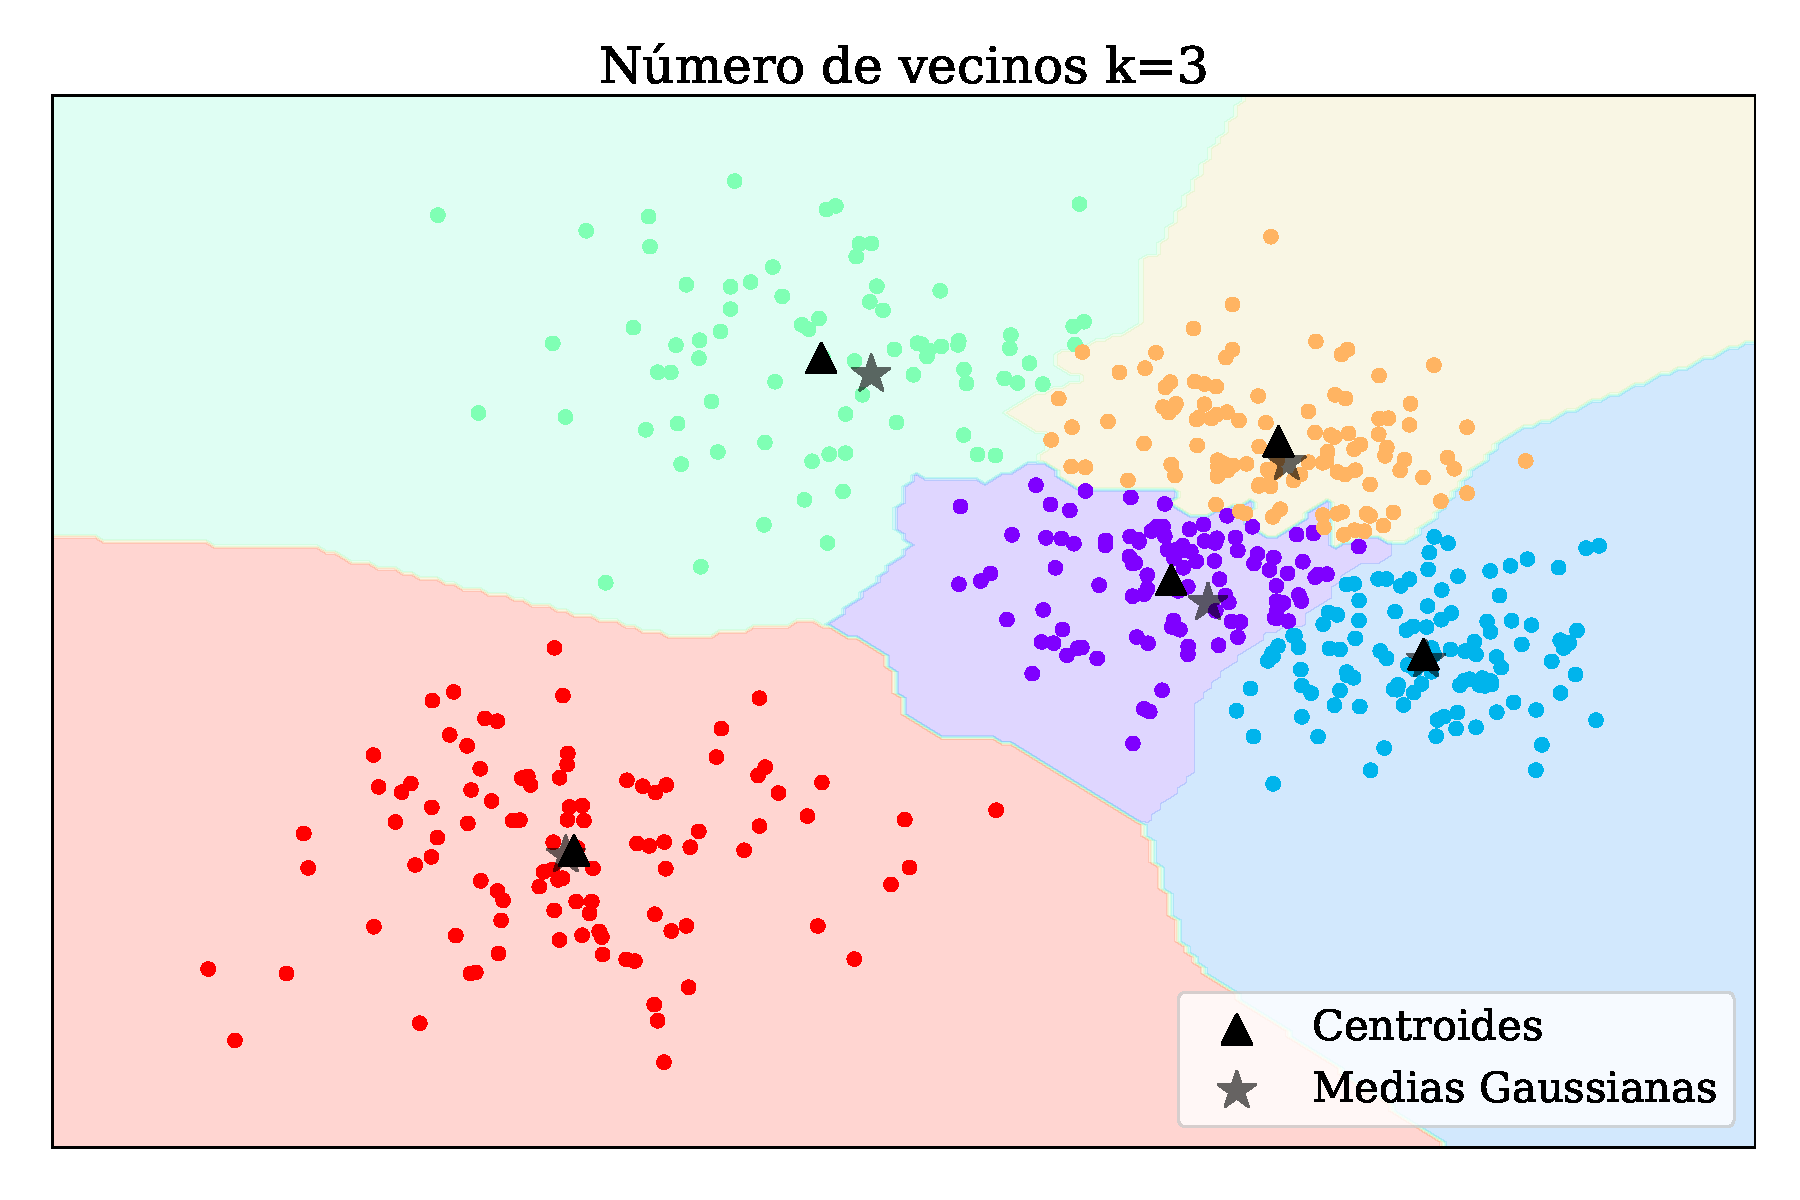
\includegraphics[width=0.5\textwidth]{plots/ejer_4_K-3_si_converge.pdf}
    \caption{K=3 }
    \label{fig:ejer4_k_3}
\end{figure} 

k=7
Dimensiones del set de entrenamiento  (375, 2)
375 ejemplos de entrenamiento
125 ejemplos para probar

72.0\% probando con 125 ejemplos
\begin{figure}[H]
    \centering
    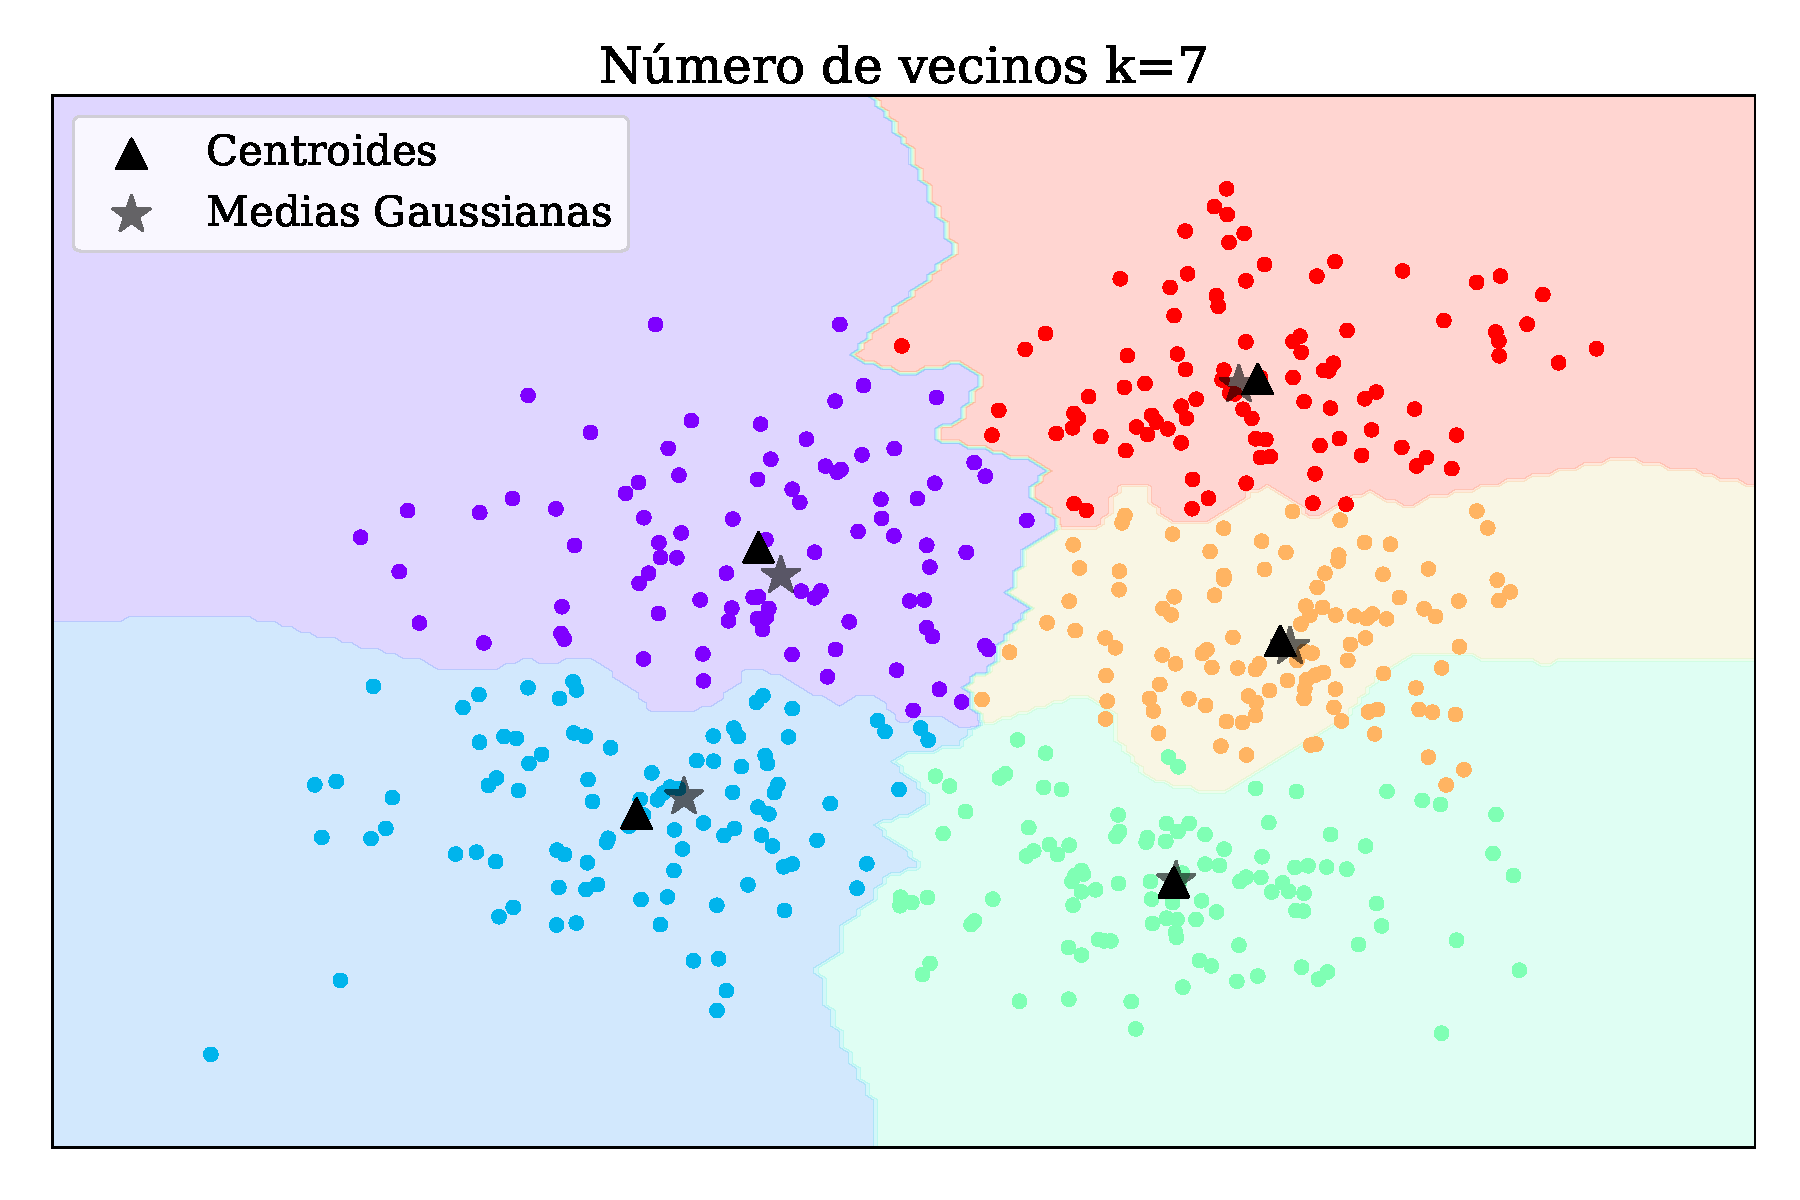
\includegraphics[width=0.5\textwidth]{plots/ejer_4_K-7_si_converge.pdf}
    \caption{K=7 }
    \label{fig:ejer4_k_7}
\end{figure} 

\section*{Ejercicio 5}

\begin{figure}[H]
    \centering
    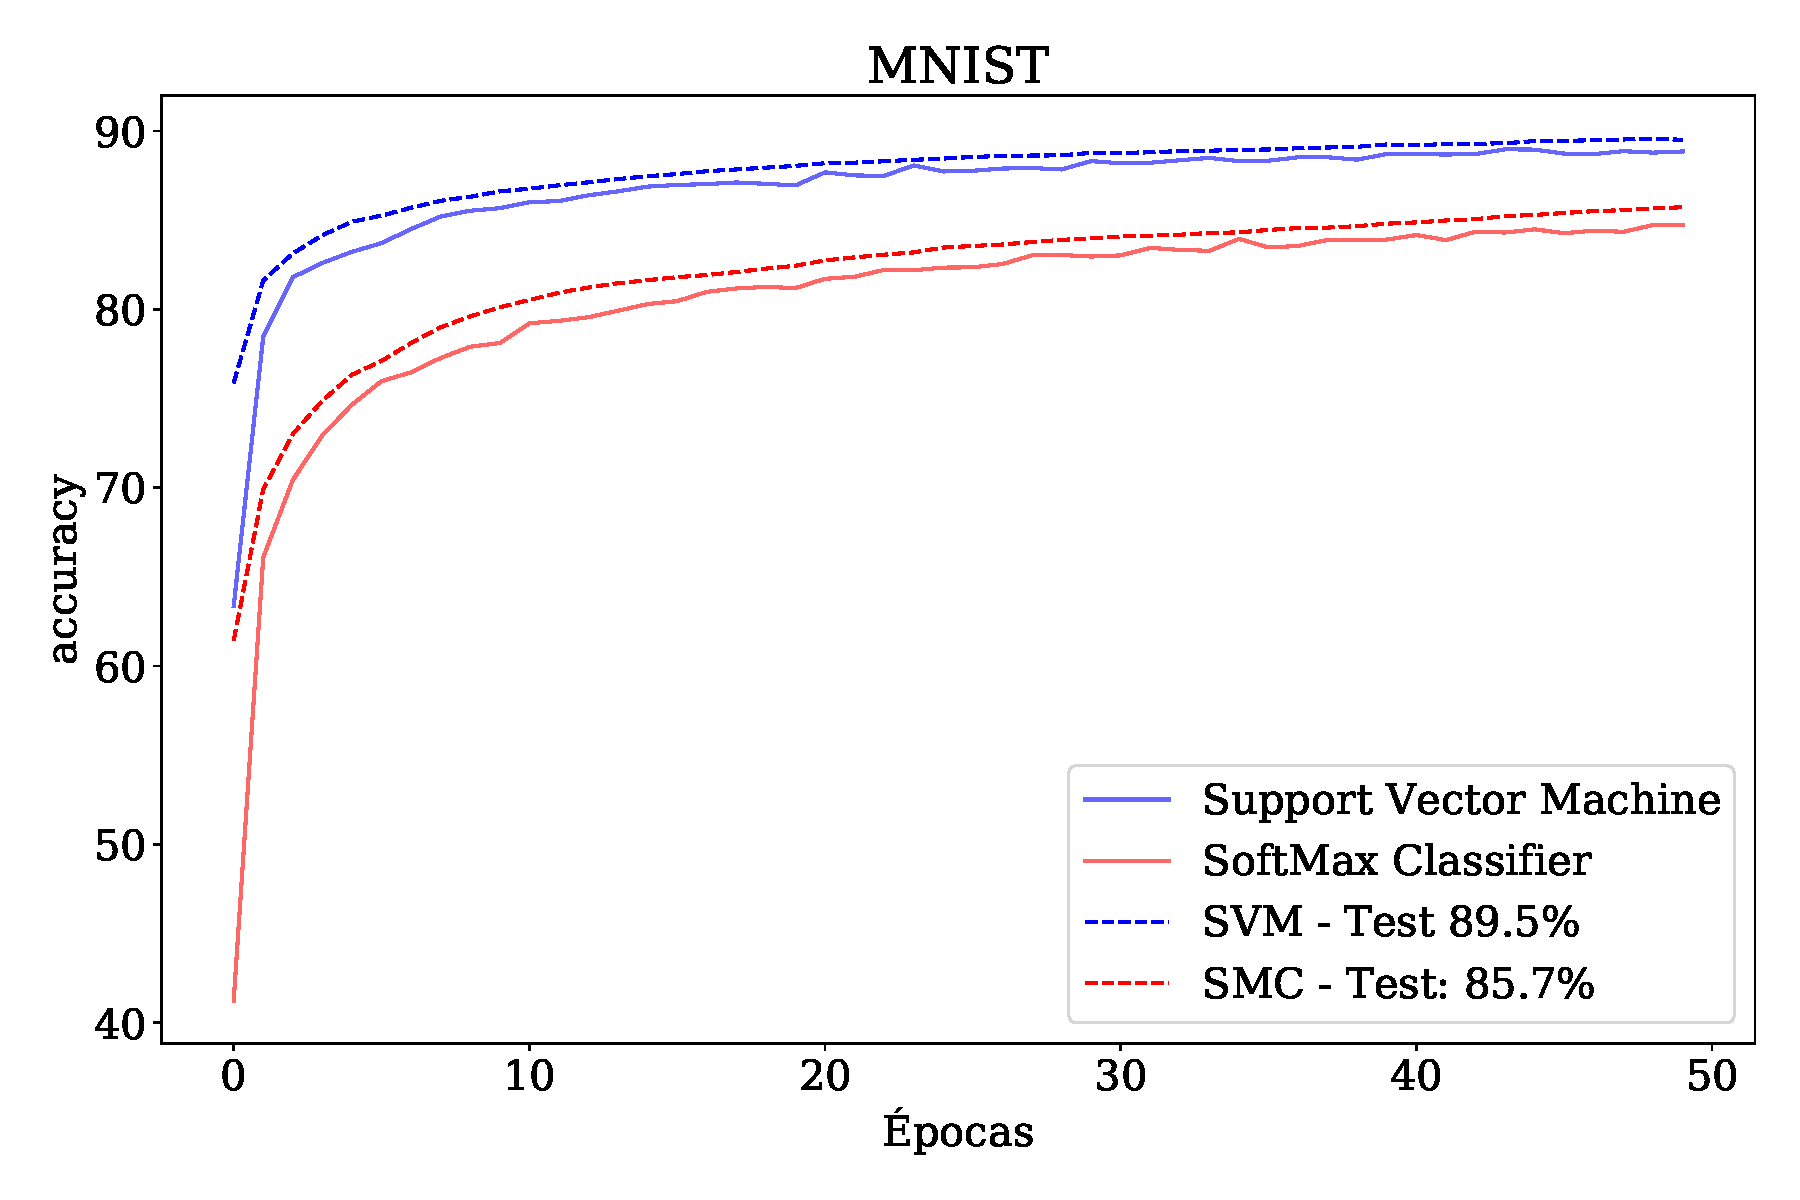
\includegraphics[width=0.5\textwidth]{plots/ejer_5_MNIST_acc.pdf}
    \caption{accuracy}
    \label{fig:ejer5_mnist_acc}
\end{figure} 

\begin{figure}[H]
    \centering
    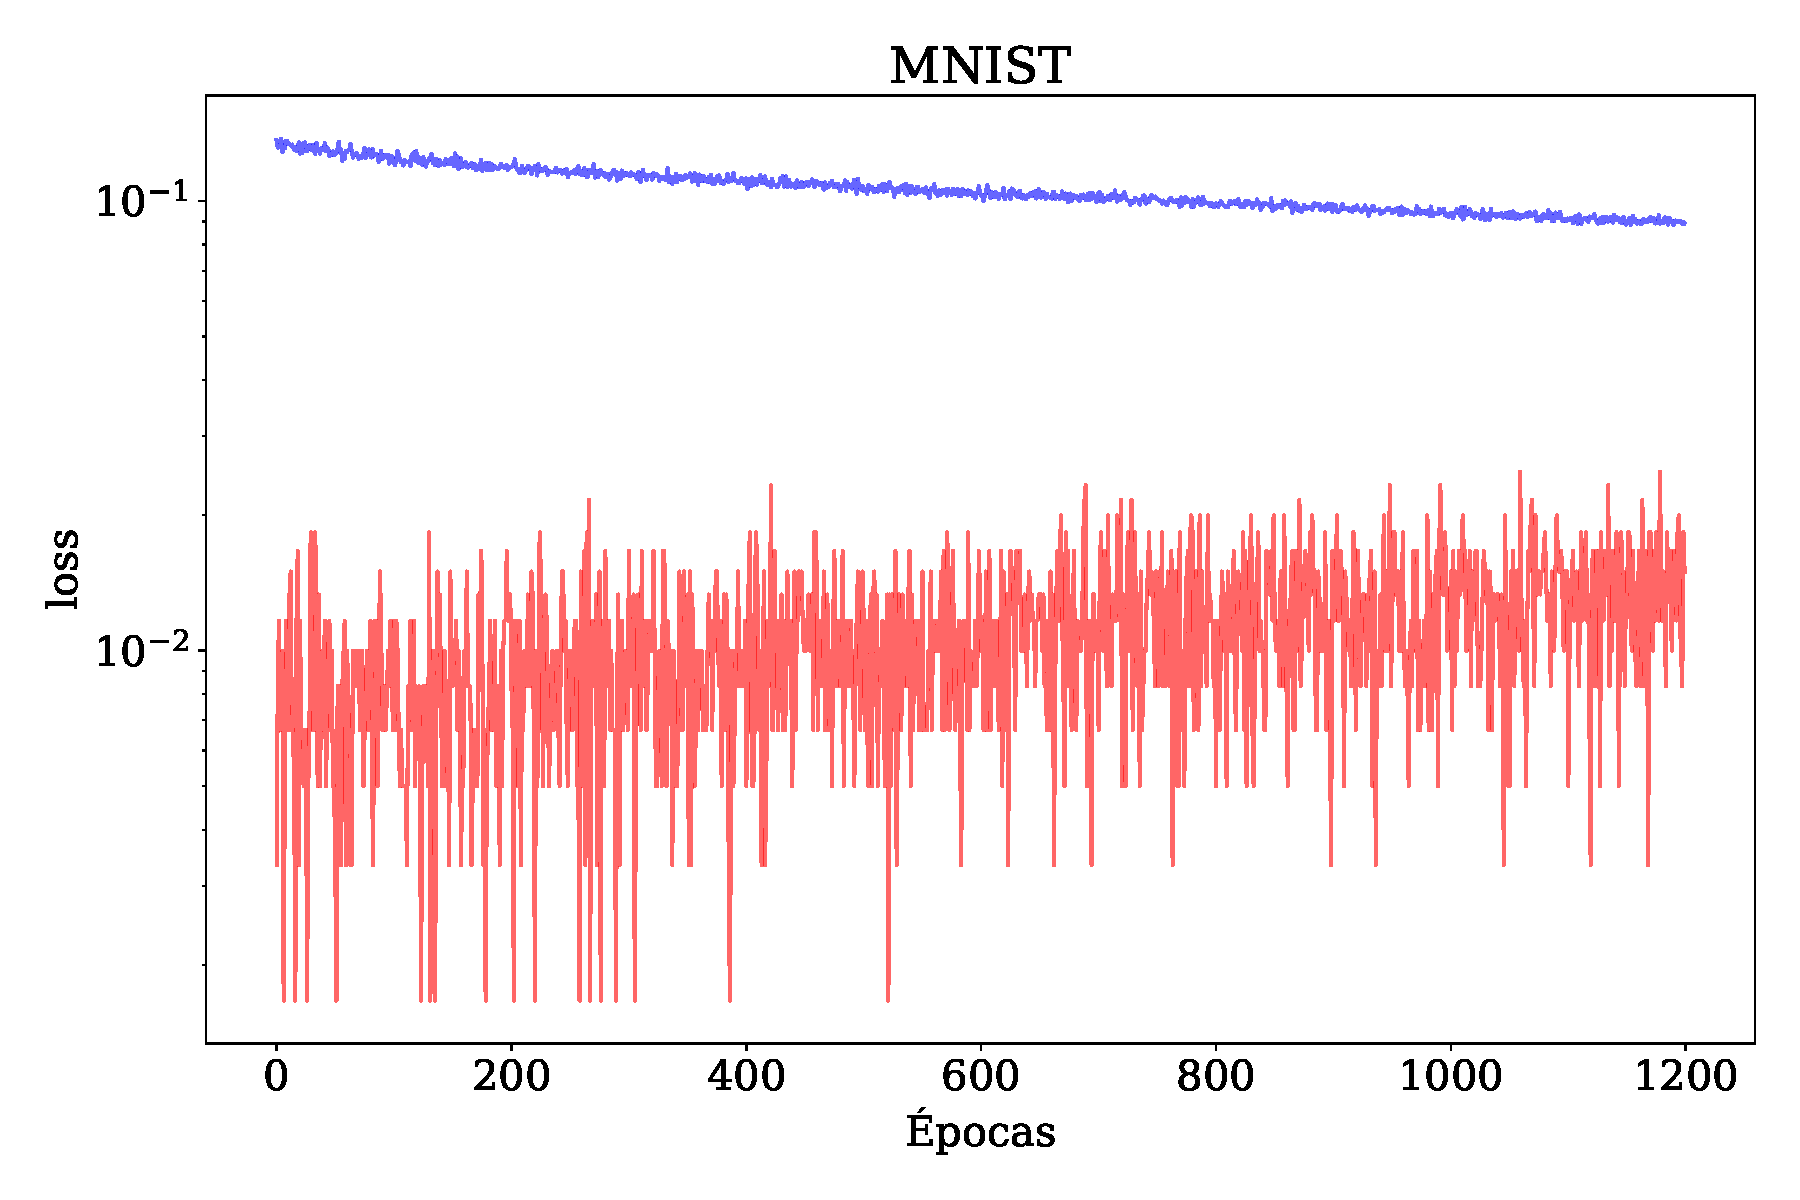
\includegraphics[width=0.5\textwidth]{plots/ejer_5_MNIST_los.pdf}
    \caption{loss}
    \label{fig:ejer5_mnist_loss}
\end{figure} 




\end{document}